%
%\addtocontents{toc}{\newpage}
\chapter{Compton Reconstruction}

\section{The physics of Compton scattering}

\begin{figure}
    \centering
    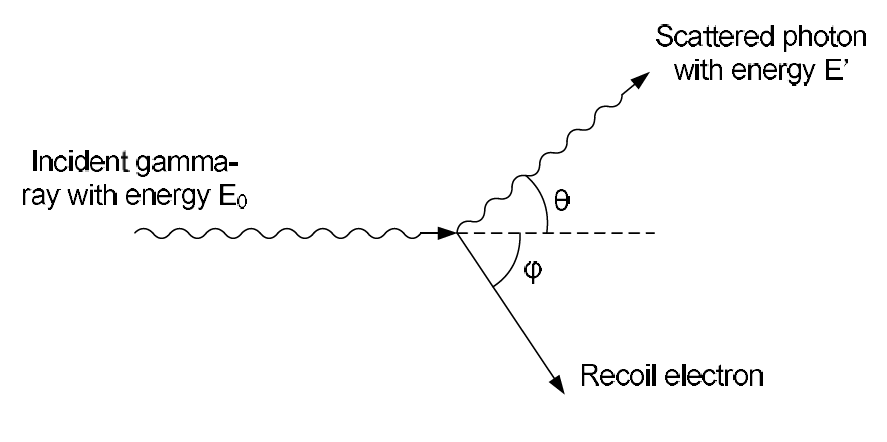
\includegraphics[width=0.7\textwidth]{Compton_scatter.png}
    \caption{Diagram of Compton scattering process. \cite{comptonThesis}}
    \label{fig:compton_scatter}
\end{figure}

Compton scattering is a process in which a photon hits a charged particle and bounces off it with a different energy and direction than it had initially. In the APT, gamma rays from space scatter off of electrons in the detector material and kick them out of the layer that they had previously been bound to. The electron and photon then move in different directions, obeying the conservation of momentum and energy, as shown in figure \ref{fig:compton_scatter}. The gamma ray's energy can then be described with this equation:

\begin{equation}
    \label{eq:compton}E' = \frac{E_0}{1+\frac{E_0}{m_ec^2}(1-\cos\theta)}
\end{equation}

Where $E'$ is the energy after the collision, $E_0$ is the energy before the collision, $\theta$ is the scattering angle of the photon, and $m_e$ is the mass of the electron. Notice that the scattering angle, the initial energy, and the final energy are the only variables in this equation, so determining any two of these values also determines the third.

These calculations are based on the assumption that the photon is at rest in the detector material prior to the collision. The effects of the electron's initial momentum lead to a phenomenon called Doppler Broadening, which causes some error in our calculations. However, this effect is very small ***(still need to find out how small) and randomly distributed, so we do not take it into account in our energy calculations.

% \section{Photon Detection} can expand if low on text

\section{Reconstructing photon direction}

\begin{figure}
    \centering
    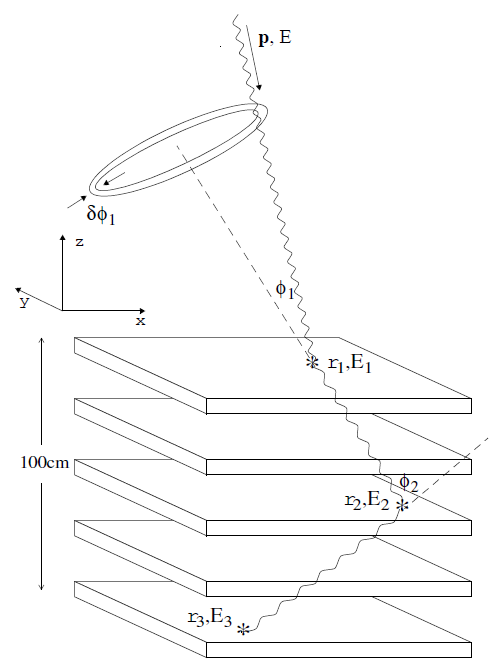
\includegraphics[width=0.5\textwidth]{detector_scattering.PNG}
    \caption{An example photon trajectory through the detector layers. Each * symbol is one hit. The dotted line shows the center of the cone of possibility while the wavy line represents the true path of the gamma-ray. \cite{comptonThesis}}
    \label{fig:scatters}
\end{figure}

Photons are detected in the APT as a series of hits in the detector material - one hit for each time the photon scatters, as shown in figure \ref{fig:scatters}. Each time the photon scatters, it deposits some energy in the detector, which is recorded when the scattered electron is absorbed. It will then either scatter again or be absorbed, depositing its full energy in the last hit. From equation \ref{eq:compton}, if we know the energy before and after the first hit, we can calculate the initial scattering angle of the photon. However, this does not give us the exact trajectory of the incident photon, but rather the "cone of possibility", defined by the scattering angle and the direction of the scattered photon. We will discuss how these angles can be used to resolve a point source in a later section.

If we knew which two hits came first in the scattering sequence, we could get the scattering angle of each photon with a simple calculation. However, the biggest challenge in reconstructing a Compton scatter is the fact that the detector cannot give us the chronological ordering of hits. Each gamma-ray moves at the speed of light, and the distance between detector layers is so small that we would need a nearly impossible time resolution to determine the first two hits by time of arrival. However, equation \ref{eq:compton} allows us to find the correct ordering a different way, by comparing the physical angles between the recorded hits to the angles that are indicated by the energy deposits. If there were no other factors involved, each correct physical angle would have an exact match in energy angle, but detector noise and electronic effects mean that we must take a probabilistic approach to finding the correct sequence.

\section{Methodology}
To make things simpler for our algorithm, we break each photon's hits down into triples, one for each possible three hits. Each triple has a physical angle - for example, $\phi_2$ in figure \ref{fig:scatters} - and an energy angle, which is calculated by equation \ref{eq:compton} using the summed energy deposits of the sequence. One obstacle to our calculations is that the scattering angle does not depend on the energy deposited at the vertex of a given triple, but on the total energy of the photon both before and after the hit at the vertex. This means that we cannot calculate the energy angles individually, but always as part of a sequence. If we change the hits in the sequence before a triple, it changes the energy calculations of the triple itself. To describe these constraints mathematically, we use these equations based on those in Boggs \& Jean\cite{Boggs}:

\begin{align}
    W_i &= \frac{1}{m_ec^2}\sum_{j=i+1}^N E_j\\
    \label{eq:new_compton}\eta' &= \cos\theta' = 1+\frac{1}{W_i}-\frac{1}{W_{i+1}}\\
    \eta &= \cos\theta = \hat{r}_i \cdot \hat{r}_{i+1}\\
    \vec{r}_i &= \vec{x}_i - \vec{x}_{i-1}
\end{align}

Where $W_i$ is the unitless energy of the photon after $i$ hits in the detector ($W_0$ would be the initial/incident energy), and the photon interacts with the detector $N$ times total. Equation \ref{eq:new_compton} is just a reformulation of the original Compton equation, \ref{eq:compton}, with $\theta'$ representing the energy scattering angle at hit $i$. $\theta$ is the spatial angle of hit $i$ (previously referred to as the physical angle), and is calculated using a dot product, where $\vec{x}_i$ refers to the position of hit $i$. As finding the inverse cosine can cost us valuable computation time, we use $\eta$ and $\eta'$ to represent the cosine of the spatial and energy angles, respectively, and compare the two directly.

\subsection*{The $\chi^2$ metric}
To compare the spatial and energy angles of a given sequence of hits, we use a probability estimate given by the $\chi^2$ distribution:

\begin{equation}
    \label{eq:chi2}\chi^2 = \frac{1}{N-2} \sum_{i=2}^{N-1} \frac{(\eta_i-\eta_i')^2}{\delta\eta_i^2+\delta\eta_i'^2}
\end{equation}

Where $\eta_i$ and $\eta_i'$ represent the spatial and energy angles, respectively, and $\delta\eta_i$ and $\delta\eta_i'$ represent the error in the spatial and energy angle, respectively.

The $\chi^2$ distribution is a sum of squared Gaussian distributions, so if we assume our noise/error, $(\eta_i-\eta_i')$, has an approximately Gaussian distribution, we can use the $\chi^2$ distribution to determine how likely a given ordering of hits is. We can see by the equation that if the spatial and energy angles of any given triple match more closely, the value of $\chi^2$ will be lower, while if they are farther apart the value of $\chi^2$ will be higher. As the factors that affect our noise and error levels are very complicated, it is likely that the actual distribution is not exactly Gaussian. However, based on the Central Limit Theorem, and a reasonable assumption of the number of independent variables that can affect our angle calculations, we can say that a Gaussian is likely a good approximation for our overall error distribution.

\iffalse

This chapter describes the components of a thesis.  You need not include all
components described here, but you must follow the prescribed order for the
components you do include. Table~\ref{tab:components} lists the required and
optional components in the order that they should appear.  Your thesis should
include three main parts: the front matter, the text, and the back matter.
Each of these parts is described below.

\section{Front Matter}

The front matter includes all material that appears before the beginning of the
main text.  Number all ``front matter'' pages (except the title page and the
optional copyright page) with lower-case roman numerals, centered just above
the bottom margin.  Each of the following sections should begin on a new page.

\subsection{Title Page}

Format the title page so that it is centered vertically and horizontally on the
page with equal amounts of white space from top and bottom margins.  Include a
1.5-inch left margin and a 1-inch right margin.  Use a 12- or 14-point regular
Garamond, Times or Roman font on this page.  If you are writing a dissertation,
substitute the word ``dissertation'' wherever the word ``thesis'' appears in
this document.  The date on the title page should reflect the month and year
the degree will be awarded and should be one of the following months: December,
May, or August.  Do \uline{not} number the title page.

\begin{table}[ht]
\refstepcounter{table}
\label{tab:components}
\centering
Table \ref{tab:components}: Required and Optional Thesis Components
\addcontentsline{lot}{table}{\numberline{\ref{tab:components}}{%
	\ignorespaces Required and Optional Thesis Components
	(NOTE: If you have a multi-lined table label/title, then the 2nd and
	all additional lines should align with the first line, just like this
	one; plus, be sure that no words display to the far right hand side
	where the page numbers for your tables display, just as shown in this
	example.)}}

% Note: the \addcontentsline is a hack to force LaTeX to add a different
% entry to the text and table-of-contents.  Don't do this normally.

\vspace{0.125in}
\begin{spacing}{1}
\begin{tabular}{| c | c | c | c|}
\hline 
\textbf{Major Part} & \textbf{Thesis Component} & \textbf{Required}
 & \textbf{Optional} \\ \hline

\textbf{Front Matter} & Title Page & $\bullet$ & \\ \cline{2-4}
 & Abstract Page & $\bullet$ & \\ \cline{2-4}
 & Copyright Page & & $\bullet$ \\ \cline{2-4}
 & Dedication & & $\bullet$ \\ \cline{2-4}
 & Table of Contents & $\bullet$ & \\ \cline{2-4}
 & List of Tables & (Rqrd if used) & \\ \cline{2-4}
 & List of Figures & (Rqrd if used) & \\ \cline{2-4}
 & List of Abbreviations & & $\bullet$ \\ \cline{2-4}
 & Glossary of Nomenclature & & $\bullet$ \\ \cline{2-4}
 & Acknowledgments & & $\bullet$ \\ \cline{2-4}
 & Preface & & $\bullet$ \\ \hline

\textbf{Text} & Chapters & & $\bullet$ \\ \hline

\textbf{Back Matter} & Appendices & & $\bullet$ \\ \cline{2-4}
 & References & $\bullet$ & \\ \cline{2-4}
 & Vita & $\bullet$ & \\ \cline{2-4}
 & Short Title Page & $\bullet$ & \\ \hline
\end{tabular}
\end{spacing}
\end{table}

\subsection{Copyright Page}

Include a copyright page if you plan to copyright your thesis.  If used, the
copyright page must be unnumbered, immediately following the title page.  It
should include three lines, centered on the page with regular body text font
and spacing.  The 1$^{st}$ line should be ``copyright by'', the 2$^{nd}$ line
should contain your full name.  The 3$^{rd}$ line should contain the year the
degree is to be awarded.  Do not number the copyright page.  If you are a
Master's candidate and would like to register your claim to copyright your
thesis, you must make all arrangements independently.  Doctoral students will
complete a publishing agreement form which will give them a copyright
registration option.

\subsection{Abstract Page}

Please see important note regarding length of abstract found near the front of
this guide within the sample abstract.  Format the abstract page precisely as
done in this document.  The abstract page \uline{always} begins the document's
page numbering at ``ii''.

\subsection{Acknowledgments}

An acknowledgments section should be included..  Use it to thank those who
supported your research through contributions of time, money, or other
resources.  Type the word ``Acknowledgments'' in chapter title style at the top
of page.  If the acknowledgments fill more than one page, put the heading only
on the first page.  Number the page with a Roman numeral, centered at bottom,
sequentially following the abstract page(s) Roman numeral(s).

\subsection{Dedication}

The dedication page is optional.  If you decide to include a separate
dedication page,  make it short and center it on the page.  If included, you
should number it, placing the next logical/sequential Roman numeral at bottom
of page, centered, as shown in this sample document.

\subsection{Table of Contents}

The table of contents must include the page numbers of all chapters and
sections of your thesis.  In addition, it may include the page numbers of all
subsections.  It must also include the page numbers of all front and back
matter elements, unless otherwise specified.  Chapter titles should appear
flush left, section headings may be indented up to 0.5 inch, and subsection
headings may be indented up to 1 inch.  Chapter titles may be typed in plain or
bold font.  All titles and headings must be followed by a dot leader and a page
number.  The word ``Contents'' must appear in chapter title style at the top of
the page.  Be sure to align multi-lined chapter titles in the table of
contents.  For example, when a table of contents' chapter or section title
extends to a second line, be sure that the 1st character of the 2nd line aligns
immediately under the 1st character of the title/chapter/section name on the
line above it (i.e., as done in this sample document's table of contents, and
as specifically illustrated in the ``list of tables'' page for
table~\ref{tab:components}).  Make certain, too, that these long titles also
align nicely within the body of text, where multi-lined chapter titles or
section titles should still break at a logical point and align in a manner
allowing the titles to be read clearly without confusion.  Sometimes, for long
chapter or section titles, this will mean forcing a line break at a logical
point.  This cannot be automated, but relies on your own good judgment.  A good
example of a multi-lined title can be found at the top of
Appendix~\ref{app:english-language}; notice how the two lines are deliberately
divided helping each phrase to be read easily and fluidly.

\subsection{List of Tables}

Include a list of tables only if your thesis actually contains tables.
Format the list of tables the same way the table of contents is
formatted, but put the word ``List of Tables'' in the heading.

\subsection{List of Figures}

Include a list of figures only if your thesis actually contains
figures. Format the list of figures the same way the table of contents
is formatted, but put the word ``List of Figures'' in the heading.

\subsection{List of Abbreviations}

Include a list of abbreviations only if you use abbreviations that are
not common in your field.  Arrange the list alphabetically.  Type the
word ``List of Abbreviations'' in chapter title style at the top of the
page.

\subsection{Glossary or Nomenclature}

Include a glossary or nomenclature section only if your thesis
contains technical words that are not commonly used by people in your
field.  Type the word ``Glossary'' or ``Nomenclature'' in chapter title
style at the top of the page.  The glossary or nomenclature section
should consist of an alphabetized list of words and their definitions.

\subsection{Preface}

A preface is optional.  If you include a preface, use it to explain the
motivation behind your work.  Format the preface the same way the
acknowledgments section is formatted, but use the word ``Preface'' in the
heading.

\section{Text}

The text part of the thesis should be divided into numbered chapters, sections,
and subsections.  Use Arabic numerals for this numbering.   Divisions smaller
than subsections may be used, but they should not be labeled with numbers.
Place Arabic page numbers throughout the body of text centered just above the
bottom margin.

\section{Back Matter}

Throughout the back matter, use the same Arabic page number formatting as used
in the body of text section.

\subsection{Appendices}

Appendices may be used for including reference material that is too lengthy or
inappropriate for the thesis text.  If one appendix is included, an appendix
title is optional.  If more than one appendix is included, each one should be
titled and lettered.  In general, appendices should be formatted like chapters.
However, they may be single spaced or include photocopied material.  If
photocopied material is used, you must add page numbers at the bottom, putting
those page numbers in square brackets to indicate that they are not part of the
original document.

\subsection{References}

The reference section should follow the final appendix (or the conclusion of
the text if there are no appendices).  Type the word ``References'' in chapter
title format at the top of the page.  Single space within references and double
space between them.  More information on formatting references is included in
Chapter~\ref{cpt:citation}.

\subsection{Vita}

Including a vita page with your thesis is optional.  If you choose to include a vita
page, it should include your name, relevant academic and professional achievements,
and current month and year you will be earning your degree.  It may also include your
publications and professional society memberships.  If included, your vita should be the 
last page of your thesis.  Note: Personally identifiable information such as birth date
and place of birth should not be included on this page.

\subsection{Short Title Page}

The short title page should be prepared as described in
Appendix~\ref{app:procedures}.

\fi

%%% Local Variables: 
%%% mode: latex
%%% TeX-master: "thesis-main"
%%% End: 
